\documentclass[french]{report}
\usepackage[T1]{fontenc}
\usepackage[utf8]{inputenc}
\usepackage[french]{babel}
\usepackage{amsmath}
\usepackage{mathtools}
\usepackage{color}
\usepackage[svgnames,dvipsnames]{xcolor} 
\usepackage{soul}
\usepackage{amssymb}
\usepackage{enumitem}
\usepackage{multicol}
\usepackage[left=2cm,right=2cm,top=2cm,bottom=2cm]{geometry}
\newcommand{\mathcolorbox}[2]{\colorbox{#1}{$\displaystyle #2$}}
\usepackage{pifont}
\usepackage{pst-all}
\usepackage{pstricks}
\usepackage{delarray}
\usepackage{setspace}
\usepackage{graphicx}
\usepackage{hyperref}
\usepackage{nicematrix}
\usepackage{listings}
\usepackage{float}

\hypersetup{
	colorlinks=true,
	linkcolor=blue,
	filecolor=magenta,      
	urlcolor=cyan,
	pdfpagemode=FullScreen,
}

\usepackage{amsthm}
\newtheorem*{Rem}{Remarque}

\newenvironment{conclusion}[1]{%
	\begin{center}\normalfont\textbf{Conclusion}\end{center}
	\begin{quotation} #1 \end{quotation}
}{%
	\vspace{1cm}
}

\newcommand\pythonstyle{\lstset{
	language=Python,
	basicstyle=\ttm,
	morekeywords={self},              % Add keywords here
	keywordstyle=\ttb\color{deepblue},
	emph={MyClass,__init__},          % Custom highlighting
	emphstyle=\ttb\color{deepred},    % Custom highlighting style
	stringstyle=\color{deepgreen},
	frame=tb,                         % Any extra options here
	showstringspaces=false
}}

\lstdefinestyle{Cpp}{
	language=C++,
	tabsize=3,
	basicstyle=\ttfamily,
	keywordstyle=\color{blue}\ttfamily,
	stringstyle=\color{red}\ttfamily,
	commentstyle=\color{green}\ttfamily,
	morecomment=[l][\color{magenta}]{\#}
}

\lstdefinestyle{Python}{
	language=Python,
	tabsize=3,
	basicstyle=\ttfamily,
	keywordstyle=\color{blue}\ttfamily,
	stringstyle=\color{red}\ttfamily,
	commentstyle=\color{green}\ttfamily,
	morecomment=[l][\color{magenta}]{\#}
}

\lstset{style=Cpp}

\setlength\parindent{0pt}
\usepackage[skip=2pt]{caption}

\usepackage{fontawesome}

\usepackage{lipsum}

% Titlepage
\newcommand{\reporttitle}{Développement de méthodes hybrides éléments finis/réseaux neuronaux pour aider à la création de jumeaux chirurgicaux numériques}
\newcommand{\reportauthorOne}{Frédérique Lecourtier}
\newcommand{\reportsupervisorOne}{Michel Duprez}
\newcommand{\reportsupervisorTwo}{Emmanuel Franck}
\newcommand{\reportsupervisorThree}{Vanessa Lleras}
\newcommand{\reporttype}{Coursework}

\begin{document}

	\begin{titlepage}

	\newcommand{\HRule}{\rule{\linewidth}{0.5mm}}
	
	\begin{center}
		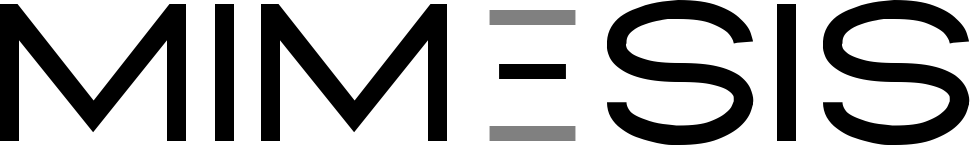
\includegraphics[width = 0.5\linewidth]{logo-mimesis.png} \\ [1.5cm] 
	
		\textsc{\Large Université de Strasbourg}\\[0.5cm] 
		\textsc{\large Rapport de Thèse}\\[0.95cm] 
		
		\HRule \\[0.4cm]
		\huge\bfseries\reporttitle\par % Title of your document
		\HRule \\[0.4cm]
	\end{center}
	
	\vspace{1cm}
	
	\begin{flushleft} \large
		\begin{minipage}{0.4\hsize}
			\textit{Auteurs:}\\
			\reportauthorOne
		\end{minipage} \hfill 
		\begin{minipage}{0.4\hsize}
			\textit{Superviseurs:}\\
			\reportsupervisorOne\\
			\reportsupervisorTwo\\
			\reportsupervisorThree
		\end{minipage}
	\end{flushleft}
	\vspace{2.5 cm}
	\makeatletter
	Date: \@date
	\hfill
	
\includegraphics[width = 0.2\linewidth]{inria.png}\\[1.5cm] 
	
	\vfill % Fill the rest of the page with whitespace
	
	\makeatother


\end{titlepage}


	\tableofcontents

	\chapter{Introduction}
	\newpage
	\graphicspath{{introduction/images/1_application}}
	\section{Domaine applicatif}
	\newpage
	\graphicspath{{introduction/images/2_contrib}}
	\section{Ma contribution}

	\chapter{Levelset}
	\newpage
	\graphicspath{{levelset/images/1_maths_theory}}
	\section{Théorie d'approximation}
	\newpage
	\graphicspath{{levelset/images/2_learning}}
	\section{Apprentissage}
\end{document}